\documentclass{article}
\usepackage[T1]{fontenc}
\usepackage{lmodern}
\usepackage{graphicx}
\usepackage{amsmath,amssymb}
\usepackage[a4paper,margin=2cm]{geometry}
\usepackage[absolute,overlay]{textpos}
\setlength{\TPHorizModule}{1mm}
\setlength{\TPVertModule}{1mm}
\usepackage[indonesian]{babel}
\usepackage{hyperref}
\setlength{\emergencystretch}{2em}
% unit: Halaman 48

\begin{document}

% === Halaman 48 (llm) ===

\begin{center}
\huge Mode Counter
\end{center}

\vspace{80mm}

\begin{tabular}{|l|l|}
\hline
CTR & \begin{aligned}
C_j &= P_j \oplus \text{E}(K, T_j) \quad j = 1, \dots, N-1 \\
C_N^* &= P_N^* \oplus \text{MSB}_u[\text{E}(K, T_N)]
\end{aligned} & \begin{aligned}
P_j &= C_j \oplus \text{E}(K, T_j) \quad j = 1, \dots, N-1 \\
P_N^* &= C_N^* \oplus \text{MSB}_u[\text{E}(K, T_N)]
\end{aligned} \\
\hline
\end{tabular}

\vspace{5mm}

$T_j$ adalah counter, nilainya bertambah satu untuk enkripsi blok berikutnya

% deskripsi: Diagram proses enkripsi dan dekripsi menggunakan Mode Counter (CTR), menunjukkan aliran data dari plaintext P ke ciphertext C melalui operasi XOR dengan hasil enkripsi counter.
% bbox normalisasi: [0.0000, 0.2600, 0.9900, 0.6400]
\begin{textblock*}{207.90mm}(0.00mm,77.22mm)
\noindent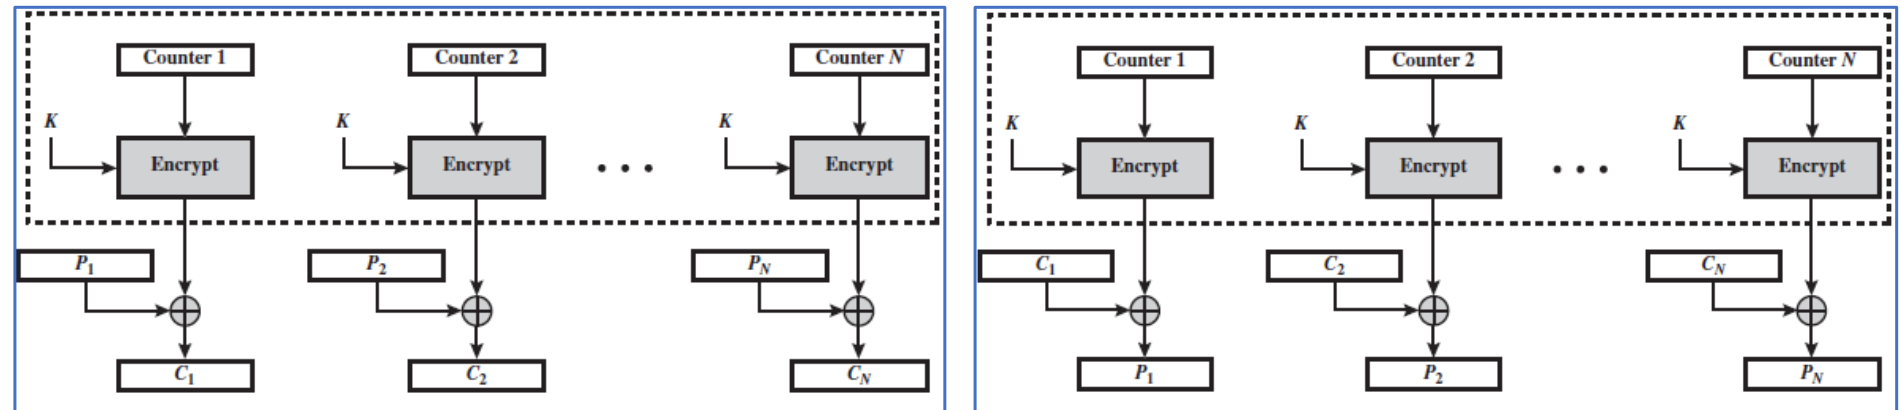
\includegraphics[width=207.90mm,height=112.86mm]{../../images/llm/page_048_img_01.png}%
\end{textblock*}

\end{document}
